%%
% Please see https://bitbucket.org/rivanvx/beamer/wiki/Home for obtaining beamer.
%%
\documentclass{beamer}
\usepackage[utf8]{inputenc}

\usetheme{Copenhagen}

\title[Horizontal and Grid Partitions]{Horizontal and Grid Partitions\\Using a DCEL with Orthogonal Polygons}
\author[João Pires, José Oliveira, DCC/FCUP]{João Rebelo Pires \and José Miguel Oliveira}
\institute[DCC/FCUP]{Departamento de Ciência de Computadores, FCUP}
\date{May 2017}

\begin{document}

\begin{frame}
\maketitle
\end{frame}

\section{The Doubly Connected Edge List Structure}
\subsection{Structure}
\begin{frame}
\frametitle{Structure}
\textbf{Attributes of a DCEL:}
\pause
\begin{itemize}[<+->]
  \item Next;
  \item Incident;
  \item Twin;
  \item Previous;
  \item Origin.
\end{itemize}
\end{frame}

\begin{frame}
\frametitle{Example}
\begin{block}{Visual Representation of a DCEL:}
	\begin{figure}
		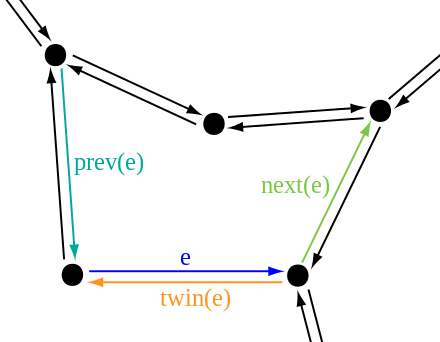
\includegraphics[scale=0.5]{images/dcel}
	\end{figure}
\end{block}

\end{frame}

\section{Horizontal Partition}
\subsection{Definition}
\begin{frame}
\begin{block}{Definition:}
	The horizontal partition of an orthogonal polygon is the partition one obtains after extending internally the horizontal edges of such polygon, until this extension intersects a vertical edge.
\end{block}
\end{frame}

\end{document}
